\chapter{Graph}

Graph merupakan sebuah \textit{Abstract Data Type} (ADT) yang digunakan untuk mengimplementasikan konsep \textit{graph} dan \textit{directed graph} dalam matematika. Dalam matematika sendiri, graph merupakan sebuah representasi dari sekumpulan objek yang saling terhubung. Objek-objek yang ada di dalam graph dikenal dengan nama \textit{vertex}, sedangkan hubungan (penghubung) antar objek tersebut dikenal dengan nama \textit{edge}.

Sebuah graph dapat digunakan untuk merepresentasikan banyak hal dalam dunia nyata. Misalnya, kita dapat merepresentasikan pohon pengetahuan dalam sebuah graph seperti yang nampak pada gambar~\ref{fig:knowledge-tree}. Peta juga kerap kali direpresentasikan sebagai graph, dengan titik-titik pergerakan sebagai vertex-nya, dan jalur antar titik sebagai edge-nya (lihat gambar~\ref{fig:map-graph}).

\begin{figure}
    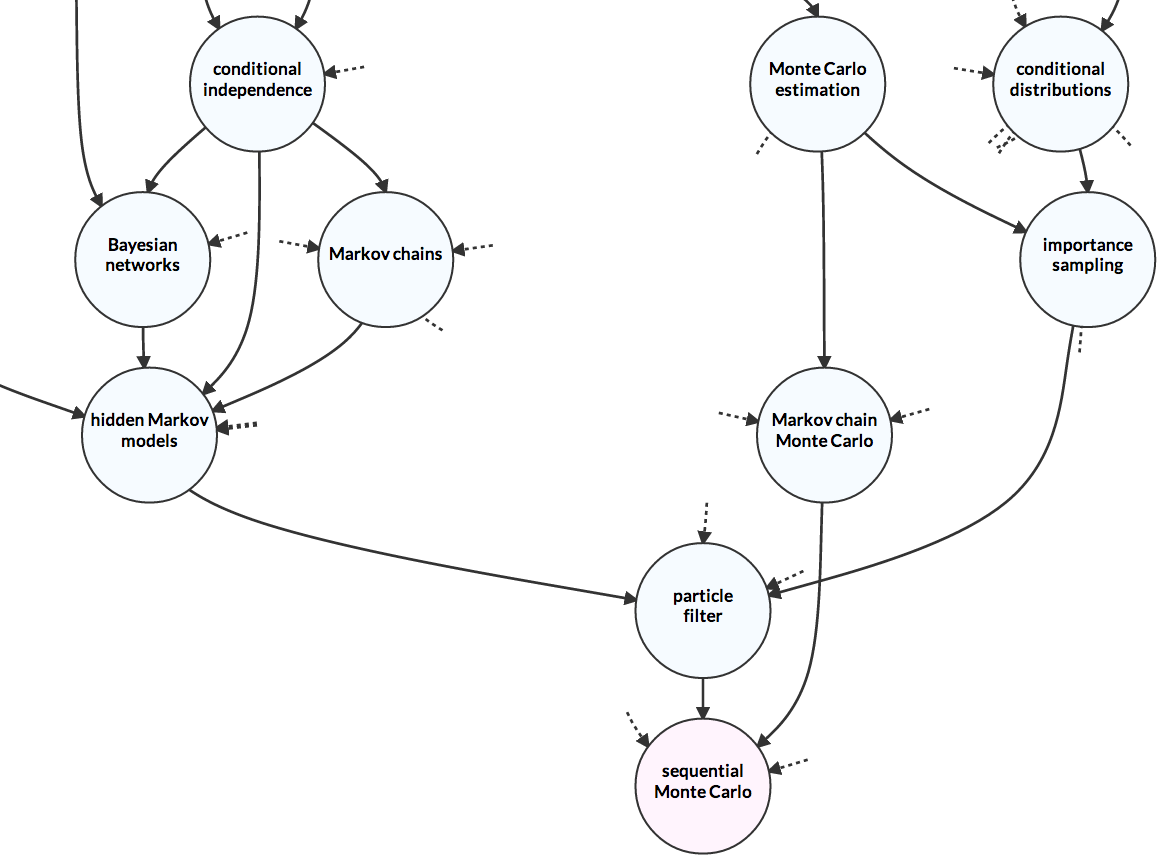
\includegraphics[width=\textwidth,keepaspectratio]{fig/KnowledgeTree.png}%
	\caption{Pohon Pengetahuan}%
	\label{fig:knowledge-tree}%
\end{figure}

\begin{figure}
    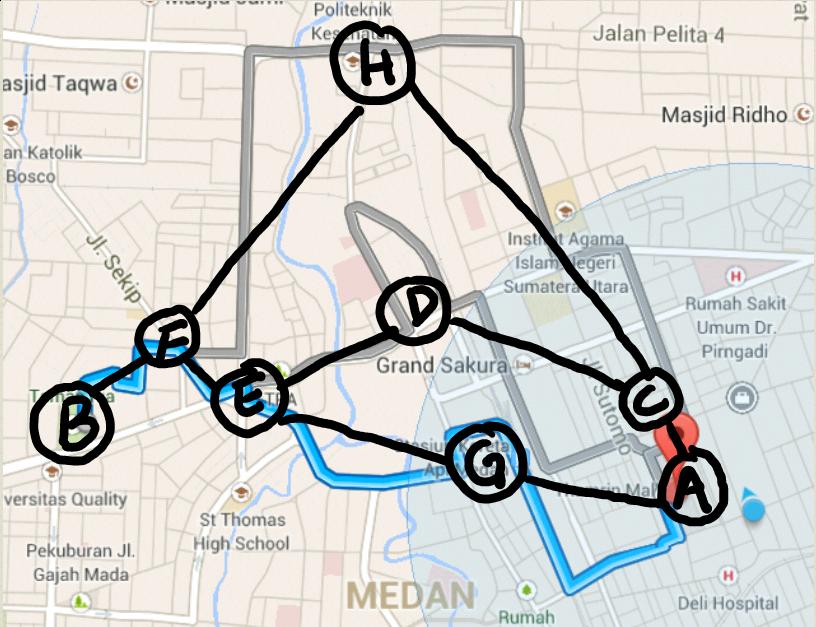
\includegraphics[width=\textwidth,keepaspectratio]{fig/DirectedGraphMap.png}%
	\caption{Peta dengan Graph}%
	\label{fig:map-graph}%
\end{figure}

Terdapat sangat banyak jenis dan definisi dari graph, yang masing-masing memiliki kegunaan spesifik dan kelebihan serta kekurangan tersendiri. Pada bagian ini kita hanya akan membahas satu jenis graph, yaitu graph tidak berarah yang berlabel. Untuk mengetahui lebih lanjut mengenai detil dari berbagai jenis graph serta kelebihan dan kekurangannya, silahkan baca buku atau modul tentang struktur data terkait.

Graph tidak berarah berlabel yang kita gunakan didefinisikan sebagai berikut:

\begin{itemize}
    \item Sebuah graph didefinisikan sebagai $G = (V, E)$.
    \item $V$ merupakan sekumpulan vertex.
    \item $E$ merupakan sekumpulan edge.
    \item $E = (V1, V2, v)$ di mana $V1$ dan $V2$ adalah dua buah vertex yang terhubung dan $v$ adalah label (bobot; jarak) dari kedua vertex tersebut.
    \item Dua buah vertex yang saling berdampingan membentuk sebuah edge dapat dihubungkand engan simbol $~$, sehingga $u ~ v$ dapat dibaca sebagai vertex $u$ dan $v$ yang berdampingan (memiliki edge).
\end{itemize}

Definisi graph yang kita gunakan tidak terlalu jauh berbeda dengan yang digunakan pada teori graph dalam matematika pada umumnya. Tetapi ingat bahwa definisi ini seringkali dimodifikasi sesuai dengan kebutuhan dan tujuan dari algoritma yang menggunakan graph tersebut. Misalnya, representasi dan definisi dari sebuah graph yang digunakan untuk menyelesaikan permasalahan pemetaan seperti mencari jalur terpendek akan berbeda dengan representasi untuk menyelesaikan masalah deteksi bahasa. Begitupun, algoritma-algoritma dasar yang sama dapat kita immplementasikan pada representasi graph yang berbeda ini (misalnya: algoritma untuk pencarian jalur terpendek). Perbedaan hanya akan ditemukan pada detil implementasi nantinya.

Untuk memperjelas pengertian tentang representasi graph yang berbeda, kita akan melihat beberapa jenis cara merepresentasikan graph yang umum digunakan.

\section{Representasi Graph}

Sebagai sebuah struktur data tingkat tinggi, kita umumnya akan membangun graph dengan menggabungkan beberapa struktur data sederhana seperti array, struktur, atau objek. Beberapa struktur data sederhana ini kemudian diintegrasikan dengan aturan tertentu agar dapat direpresentasikan sebagai graph. Secara umum terdapat tiga metode untuk merepresentasikan graph dari struktur-struktur sederhana seperti ini, yaitu:

\begin{description}
    \item[Adjacency List] \hfill \\
        Pada adjacency list, vertex direpresentasikan sebagai sebuah objek khusus (mulai dari yang sederhana seperti string sampai objek buatan sendiri). Vertex kemudian disimpan di dalam sebuah list atau array, dan setiap vertex menyimpan list atau array dari vertex yang berdampingan.
    \item[Adjacency Matrix] \hfill \\
        Pada adjacency matrix, kita menyimpan data graph di dalam sebuah matriks, dengan bagian baris sebagai vertex asal dan bagian kolom sebagai vertex tujuan. Isi dari matriks sendiri adalah jumlah edge yang menghubungkan kedua vertex (baris dan kolom). Data dari semua vertex dan edge sendiri harus di luar matriks.
    \item[Incidence Matrix] \hfill \\
        Pada incidence matrix, graph direpresentasikan dalam matriks dua dimensi, dengan baris matriks sebagai vertex dan kolom matriks sebagai edge. Nilai dari matriks mengindikasikan keterhubungan (\textit{incidence}) antara vertex dengan edge.
\end{description}

Untuk melihat detil yang dijabarkan, mari kita lihat masing-masing representasi ini dengan lebih mendalam.

\subsection{Graph dengan Adjacency List}

\subsection{Graph dengan Adjacency Matrix}

\subsection{Graph dengan Incidence Matrix}

\section{Operasi Umum Graph}

Terdapat beberapa operasi umum yang dapat dilakukan terhadap graph, yaitu:

\begin{enumerate}
    \item Penambahan Vertex baru
    \item Penambahan Edge baru
    \item Penghapusan Vertex
    \item Penghapusan Edge
    \item Pengecekan apakah dua buah vertex terhubung
\end{enumerate}

Kompleksitas dari masing-masing operasi sendiri berbeda-beda, tergantung dari cara representasi graph yang kita gunakan

\section{Contoh Implementasi Graph}

Implementasi graph dapat dimulai dari pembuatan sebuah kelas untuk graph seperti yang dapat dilihat pada algoritma~\ref{algo:migraph-class}.

\lstinputlisting[language=Python, 
                 firstline=1,
                 lastline=1,
                 label={algo:migraph-class},
                 caption=Definisi Kelas MiGraph
                ]
                {code/migraph.py}

Struktur graph sendiri disimpan ke dalam sebuah variabel privat, yang adalah sebuah \textit{dictionary}. Pembuatan struktur internal graph ini dibuat pada saat objek dibuat. Pengguna juga dapat memberikan graph sesuai dengan struktur internal, seperti yang tampak pada algoritma~\ref{algo:migraph-constructor}.

\lstinputlisting[language=Python, 
                 firstline=16,
                 lastline=17,
                 label={algo:migraph-constructor},
                 caption=Definisi Constructor MiGraph
                ]
                {code/migraph.py}

Pengambilan seluruh vertex dan edge yang ada dapat dilakukan dengan cukup gamblang: hanya mengubah kunci dictionary menjadi list untuk vertex, dan menelusuri isi value dari dictionary untuk edges. Algoritma~\ref{algo:migraph-vertices-edges} menunjukkan cara kerja dari bagian pengambilan seluruh vertex dan edge.

\lstinputlisting[language=Python, 
                 firstline=19,
                 lastline=30,
                 label={algo:migraph-vertices-edges},
                 caption=Pengambilan Seluruh Vertex dan Edge
                ]
                {code/migraph.py}

Karena cara penyimpanan adjacent list yang menyimpan semua vertex tetangga di dalam key dictionary, kita dapat mengecek apakah sebuah vertex bertetangga dengan vertex lain dengan sangat mudah. Algoritma~\ref{algo:migraph-is-adjacent} memperlihatkan implementasi fungsi untuk pengecekan apakah vertex bertetangga dengan vertex lainnya.

\lstinputlisting[language=Python, 
                 firstline=32,
                 lastline=33,
                 label={algo:migraph-is-adjacent},
                 caption=Cek Apakah $v1$ dan $v2$ Bertetangga
                ]
                {code/migraph.py}

Penambahan vertex dan edge juga dapat dilakukan dengan sangat sederhana: tambahkan nilai baru di dalam dictionary atau list sesuai dengan kebutuhan. Algoritma~\ref{algo:migraph-add-vertex-edge} memperlihatkan cara implementasi fungsi penambahan vertex dan edge.

\lstinputlisting[language=Python, 
                 firstline=35,
                 lastline=56,
                 label={algo:migraph-add-vertex-edge},
                 caption=Penambahan Vertex dan Edge
                ]
                {code/migraph.py}

Pengambilan vertex yang ada di sekitar vertex sendiri dilakukan dengan cara yang sama dengan pengambilan vertex: hanya mengubah key menjadi list. Algoritma~\ref{algo:migraph-get-neighbour} menunjukkan langkah yang digunakan.

\lstinputlisting[language=Python, 
                 firstline=58,
                 lastline=68,
                 label={algo:migraph-get-neighbour},
                 caption=Pengambilan Vertex Sekitar
                ]
                {code/migraph.py}

Penghapusan vertex maupun edge dilakukan dengan cara yang sama dengan penambahan dan pengambilan nilai vertex, yaitu sesuai dengan semantik python. Algoritma~\ref{algo:migraph-remove-vertex-edge} menunjukkan langkah yang digunakan.

\lstinputlisting[language=Python, 
                 firstline=70,
                 lastline=78,
                 label={algo:migraph-remove-vertex-edge},
                 caption=Penghapusan Vertex dan Edge
                ]
                {code/migraph.py}

